\begin{scanpage}{0026}{9}
\begin{center}\begin{minipage}[t]{.48\linewidth}\vspace{0pt}\centering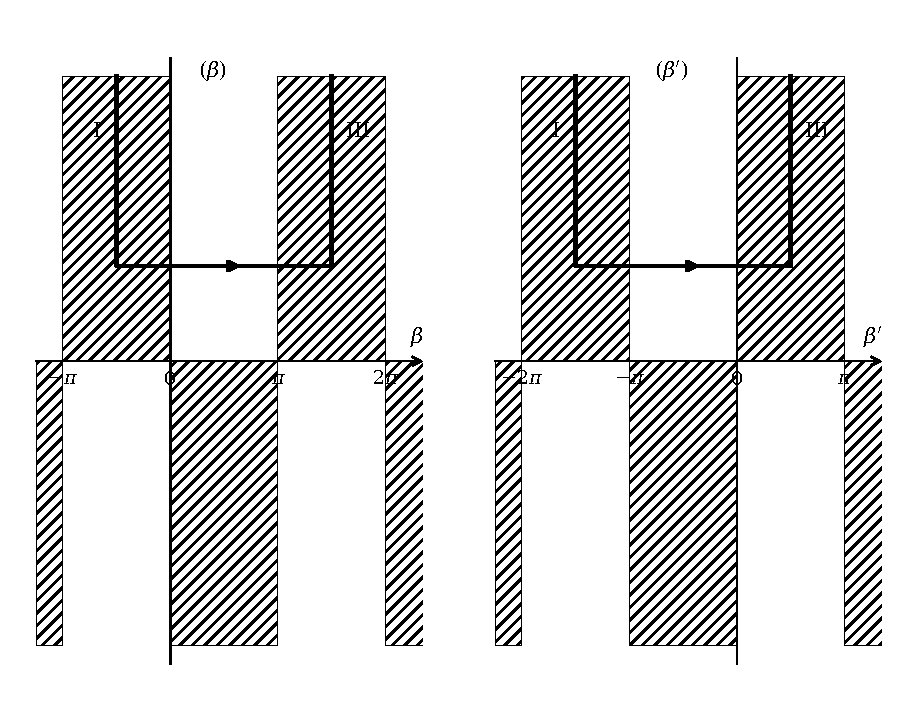
\includegraphics[width=.98\linewidth,height=5cm,keepaspectratio]{images/recreated/a-0026-fig2.pdf}\par Figure 2. The integration contours in the complex plane $\beta$.\end{minipage}\hfill\begin{minipage}[t]{.48\linewidth}\vspace{0pt}\centering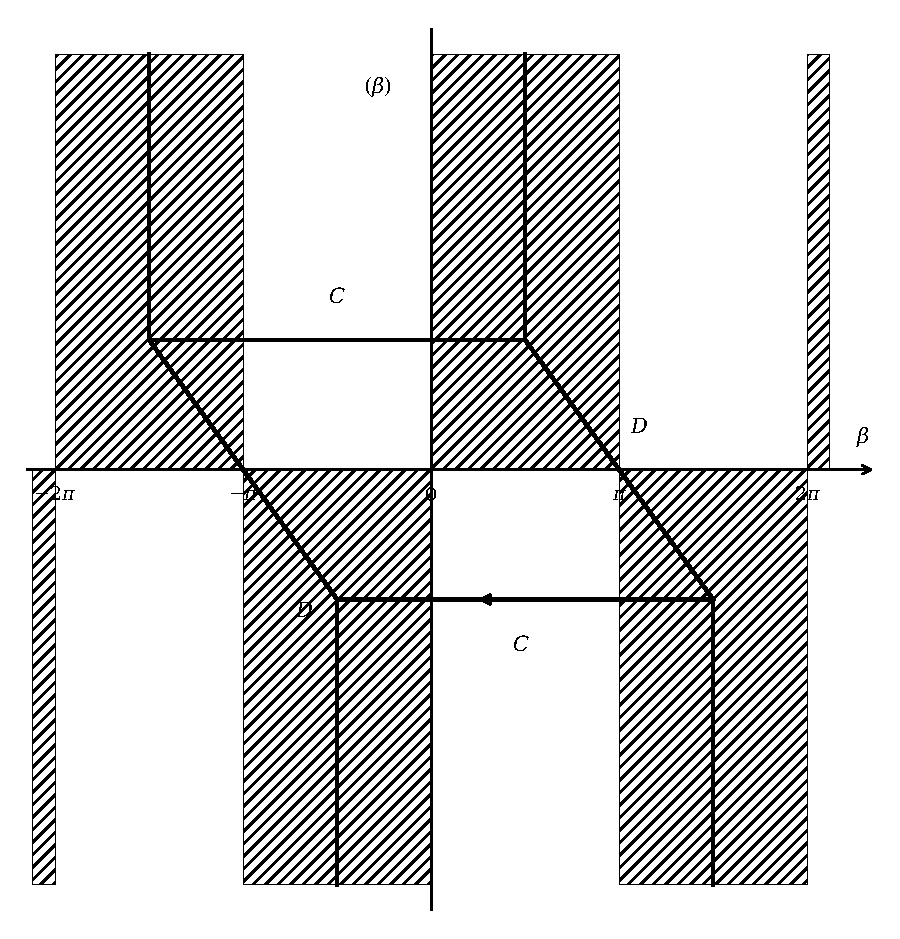
\includegraphics[width=.98\linewidth,height=5cm,keepaspectratio]{images/recreated/a-0026-fig3.pdf}\par Figure 3. The integration contour in Equation (1.28).\end{minipage}\end{center}
As a result, we obtain the well-known integral of Sommerfeld
\[u(r,\psi)=\frac1{2\alpha}\int_C\frac{e^{-ikr\cos\beta}}{1-e^{i\frac\pi\alpha(\beta+\psi)}}\,d\beta.\tag{1.28}\]
The integration contour $C$ is shown in Figure 3 and consists of two infinite branches. Since the integrand expression has poles at the points $\beta_m=2\alpha m-\psi$ $(m=0,\pm1,\pm2,\ldots)$, then for the values of $\phi$ corresponding to the space outside the wedge $(0<\phi<\alpha)$ the function $u(r,\psi)$ may be represented (with $\pi<\alpha\leq2\pi$, $0\leq\phi_0\leq\pi$) in the following way:
\[\left.\begin{aligned}u(r,\psi)&=v(r,\psi)+e^{-ikr\cos\psi}&&\text{with }-\pi<\psi<\pi,\\u(r,\psi)&=v(r,\psi)&&\text{with }\pi<\psi<2\alpha-\pi,\\u(r,\psi)&=v(r,\psi)+e^{-ikr\cos(2\alpha-\psi)}&&\text{with }2\alpha-\pi<\psi<2\alpha,\end{aligned}\right\}\tag{1.29}\]
where
\[v(r,\psi)=\frac1{2\alpha}\int_D\frac{e^{-ikr\cos\beta}}{1-e^{i\frac\pi\alpha(\beta+\psi)}}\,d\beta.\]
\end{scanpage}
